\documentclass[11pt]{article}
\usepackage[a4paper, total={6.8in, 9.25in}]{geometry}
\usepackage{graphicx}
\graphicspath{ {./assets/images/output/} }
\usepackage{caption}
\usepackage[english]{babel}
\usepackage{titling}
\usepackage{float}
\usepackage{amsmath}
\usepackage{minted}
\usepackage{multicol}
\usepackage{array}
\usepackage{setspace}
\usepackage{placeins}
\usepackage{tabularx}
\usepackage{booktabs}

% \usepackage{lipsum}

\title{Implementation of Dynamic Routing using Routing Information Protocol (RIP)}
\author{}
\date{}

\pagenumbering{gobble}
\begin{document}
\input{cn_cover.tex}

\pagebreak

\tableofcontents

\pagebreak
\pagenumbering{arabic}
\maketitle

\section{Theory and Introduction}
Routing is the fundamental process of directing data packets across an interconnected network from a source node to a destination node through various intermediate devices. This experiment focuses on the Network Layer (Layer 3) of the Open Systems Interconnection (OSI) model \cite{tanenbaum2021}. While static routing is effective for small, unchanging topologies, it becomes administratively burdensome as networks scale.

Dynamic routing addresses this by allowing routers to automatically exchange information about the network topology. The Routing Information Protocol (RIP) is a distance-vector protocol that utilizes the Bellman-Ford algorithm to determine the best path based on hop count.

In this experiment, RIP was implemented. RIP supports Variable Length Subnet Masking (VLSM) and utilizes multicast addressing for routing updates, which prevents unnecessary processing by non-routing devices on the network \cite{stallings2013}.

% --- Methodology ---
\section{Methodology}
The experiment was conducted using Cisco Packet Tracer (Version 9.0) \cite{packettracer2026}. The topology from the previous experiment was extended and converted to a dynamic routing environment through the following steps:

\begin{itemize}
    \item \textbf{Topology Extension:} A fourth router (Router 3) and a corresponding LAN were integrated into the existing network. New serial links were established to connect Router 2 to Router 3.
    \item \textbf{Removal of Static Routes:} All previously configured manual routes were deleted using the \texttt{no ip route} command to ensure that the dynamic protocol had full control over the routing table.
    \item \textbf{RIP Activation:} The dynamic routing process was initiated on all routers using the \texttt{router rip} command. The version was explicitly set to \texttt{version 2}.
    \item \textbf{Network Advertisement:} Each router was configured to "advertise" its directly connected networks using the \texttt{network} command. For example, Router 0 advertised 10.0.0.0 and 40.0.0.0.
    \item \textbf{Verification:} Connectivity was verified across all four subnets using the \textit{Ping} and \textit{Tracert} utilities to ensure the routers had successfully synchronized their tables.
\end{itemize}

% --- Results ---
\section{Results}
The comprehensive addressing scheme for the extended network is summarized in Table 1.

\begin{table}[h!]
    \centering
    \caption{Extended Network Addressing Table (RIPv2)}
    \begin{tabular}{@{}lllll@{}}
        \toprule
        \textbf{Device} & \textbf{Interface} & \textbf{IPv4 Address} & \textbf{Subnet Mask} & \textbf{Default Gateway} \\ \midrule
        Router 0        & Fa0/0              & 10.10.10.0            & 255.0.0.0            & N/A                      \\
        Router 0        & Se2/0              & 40.40.40.1            & 255.0.0.0            & N/A                      \\
        Router 1        & Fa0/0              & 20.20.20.0            & 255.0.0.0            & N/A                      \\
        Router 1        & Se2/0              & 40.40.40.2            & 255.0.0.0            & N/A                      \\
        Router 1        & Se3/0              & 50.50.50.1            & 255.0.0.0            & N/A                      \\
        Router 2        & Fa0/0              & 30.30.30.0            & 255.0.0.0            & N/A                      \\
        Router 2        & Se2/0              & 50.50.50.2            & 255.0.0.0            & N/A                      \\
        Router 2        & Se3/0              & 70.70.70.1            & 255.0.0.0            & N/A                      \\
        Router 3        & Fa0/0              & 60.60.60.0            & 255.0.0.0            & N/A                      \\
        Router 3        & Se2/0              & 70.70.70.2            & 255.0.0.0            & N/A                      \\
        PC 11           & NIC                & 10.10.10.1            & 255.0.0.0            & 10.10.10.0               \\
        Laptop 12       & NIC                & 10.10.10.2            & 255.0.0.0            & 10.10.10.0               \\
        PC 21           & NIC                & 20.20.20.1            & 255.0.0.0            & 20.20.20.0               \\
        Laptop 22       & NIC                & 20.20.20.2            & 255.0.0.0            & 20.20.20.0               \\
        PC 31           & NIC                & 30.30.30.1            & 255.0.0.0            & 30.30.30.0               \\
        PC 32           & NIC                & 30.30.30.2            & 255.0.0.0            & 30.30.30.0               \\
        PC 41           & NIC                & 60.60.60.1            & 255.0.0.0            & 60.60.60.0               \\
        Laptop 42       & NIC                & 60.60.60.2            & 255.0.0.0            & 60.60.60.0               \\ \bottomrule
        \bottomrule
    \end{tabular}
\end{table}

\begin{figure}[H]
    \centering
    
\includegraphics[width=\textwidth]{network.png}
    \caption{Extended Topology with 4 Routers and Dynamic RIP Routing}
\end{figure}

\begin{figure}[H]
    \centering
    
\includegraphics[width=0.68\textwidth]{ip_route.png}
    \caption{Routing Table showing RIP Learned Routes (Marked with 'R')}
\end{figure}

% --- Discussion ---
\section{Discussion}
The primary observation in this experiment was the efficiency of network convergence. Upon adding the 70.0.0.0 network, the information propagated automatically through the neighbors. As demonstrated in Figure 2, the routing table entries were updated to reflect the new topology without manual intervention.

\begin{figure}[H]
    \centering
    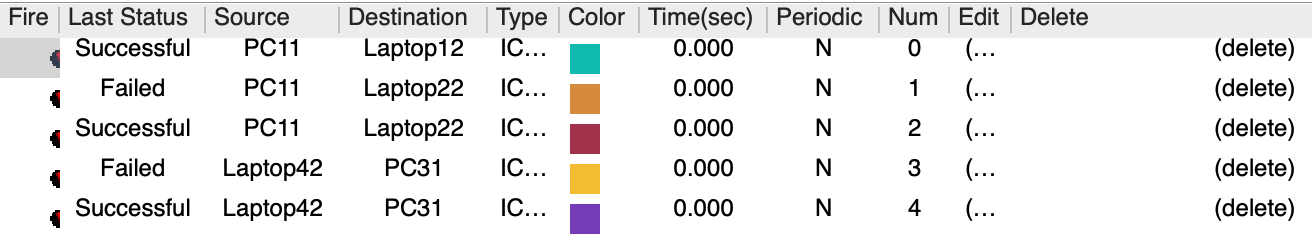
\includegraphics[width=0.68\textwidth]{ping.png}
    \caption{Verification of End-to-End Connectivity via Successive ICMP Requests}
\end{figure}

In the \textit{tracert} analysis from PC11 to PC41, the packet traversed three intermediate routers. This confirmed that RIP correctly calculated the shortest path based on the minimum hop count. The "Initial Failure" phenomenon was again observed due to ARP resolution (Figure 3), but subsequent communication was seamless. This experiment highlights that while RIPv2 is limited by a maximum hop count of 15, its ease of configuration makes it superior to static routing for expanding networks.

% --- Conclusion ---
\section{Conclusion}
The implementation of dynamic routing using RIPv2 was successfully achieved. The experiment demonstrated the protocol's ability to automate routing table updates and manage multi-hop communication without manual path definition. By comparing this to the previous static routing lab, the scalability and reduced administrative overhead of dynamic protocols were clearly observed.

\bibliographystyle{IEEEtran}
\renewcommand{\bibname}{References}
\addcontentsline{toc}{section}{References}
\bibliography{ref}

\end{document}
